\chapter{Background}\label{chapter:background}

% \Zeb{Argument of thesis is that it is important to explore the phonemic representation. In \cref{sec:12-inputrepresentations} I define ``input representation'', establishing a contrast between the default and phoneme input representation. Review past work on input representation in language models and recent work on tokenisation methods, concluding that the phoneme input representation is largely under-studied in the modern NLP landscape. In \cref{sec:12-phoneval} I review work regarding phonological evaluation of language models. This includes the use of the phoneme input representation in early connectionist models of language processing and computational models of acquisition as well as more recent work using phonemes in language models to study phonology cross-lingually to benchmarks that directly probe the phonological capabilities of LMs. Finally, in \cref{sec:12-babylm} I review work concerning the use of developmentally-plausible language models. Such models provide a useful framework for studying linguistic theories but mostly continue to use the default input representation, despite children not learning from arbitrary subwords. This chapter concludes that there is a clear need to study the use of the phoneme input representation in modern LM architectures.}

%CHAT: Language models (LMs) are systems that assign probabilities to sequences of linguistic units, such as words, characters, or phonemes. While architectural advances have received significant attention, the form of the input representation—how raw linguistic data is encoded for the model—remains a foundational and sometimes under-examined design decision. This chapter focuses on input representation, defined here as comprising three main components: modality (e.g. orthographic, phonemic), tokenisation, and pre-processing.
%Two major input paradigms are considered: subword-based input representations, which are now dominant in large-scale language modelling, and phoneme-based input representations, which provide an alternative aligned more closely with speech and cross-linguistic structure. Section 2 traces the historical development of input design choices across architectures. Sections 3 and 4 present each input paradigm in detail. Sections 5 and 6 examine their implications for phonological modelling and cognitive plausibility.
%A language model (LM) is a computational system that assigns probabilities to sequences of linguistic units, typically words, characters, or phonemes. Formally, given a sequence .. Language models can be used for generation, prediction, or as pre-trained components for downstream tasks. The input to a language model—referred to here as the input representation—is the focus of this chapter.

\defn{Language models} are statistical models of (natural) language that assign probabilities to sequences of linguistic units, such as words, characters or phonemes. While architectural advancements have received significant attention, the form of the \defn{input representation} --- how raw linguistic data is encoded for the model --- remains a foundational and under-examined design decision. Input representations are defined here as compromising three main components:

\begin{itemize}
    \item \textbf{Modality:} The modality of the raw data (e.g. orthographic text, phonemic transcriptions, audio).
    \item \textbf{Pre-processing:} Specific operations to clean the raw data, such as lowercasing or punctuation. 
    \item \textbf{Tokenisation:} How the pre-processed raw data is split into discrete tokens.
\end{itemize}

This thesis adopts a distinction between two broad types of input representation. The \defn{subword-based input representation} refers to the use of orthographic text, segmented into subword units, with whitespace-preserved word boundaries --- a representation that currently dominates large-scale language modelling. In contrast, the \defn{phoneme-based input representation} uses a phonemic modality for the raw data, removes explicit word boundaries and treats individual phonemes as atomic units. This representation has roots in computational models of language processing, speech recognition technology and phonological experimentation, but has rarely been examined in modern language model architectures --- the topic of this thesis.

This chapter provides the necessary background to understand the contrast between these paradigms. \Cref{sec:12-architectures} traces the historical development of input design choices across architectures. \Cref{sec:12-subword,sec:12-phonemic} present each input paradigm in detail. Finally, \cref{sec:12-plausiblepretraining} presents recent work in developmentally-plausible language modelling, a practical framework for exploring the use of a phoneme-based input representation with modern architectures.

\section{Evolution of input representations in language models}\label{sec:12-architectures}

\Zeb{Insert figure comparing segmentations for tokenisation: character, subword, word, audio, maybe showing the shift over time.}

Instead of using a grammar to determine the structure of a sentence, language models are \emph{distributional} --- they probabilities assigned to each linguistic unit in a sequence based on its context --- the ``company it keeps'' \citep{firth1957synopsis}. The standard formulation is:
\begin{align}
    P\left(w_t \mid w_1, \dots, w_{t-1} \right), \label{eq:languagemodel}
\end{align}

where $w_k$ denotes the linguistic unit at position $k$. These units are referred to as \defn{tokens} and are drawn from a set of possible tokens $\vocab$, also known as the \defn{vocabulary}. This formulation provides a convenient method for determining the probability of a sequence using the chain rule of probability:
\begin{align}
    P(w_1, \dots, w_T) = \prod_{t=1}^{T} P\left(w_t \mid w_1, \dots, w_{t-1}\right).
\end{align}


Language models of this type are called \defn{auto-regressive} since they predict the next item in a sequence based on on previous items from the same sequence. This can be leverage in language generation tasks, where sequences can be produced by iteratively sampling from the distribution $P(\cdot | w_1, \dots, w_{t-1})$.

% TODO: Possibly insert XLNet and NAR below

In recent years, the term ``language model'' has also been used to refer to models do not use the language modelling equation above. For example, masked language models \citep[MLM;][]{devlin2019bert} are trained to predict items in a sequence using bi-directional context, but typically only in order to learn contextual representations of tokens for language understanding tasks, not to estimate probabilities or generate sequences. This thesis focuses on auto-regressive models, since the use of phoneme-based input representations is primarily explored in contexts where token-level or sequence-level probabilities are required.

The choice of input representation determines how the tokens represent natural language. The tokenisation includes the granularity (e.g. words vs characters), the modality (e.g. phonemes vs graphemes) and whether pre-processing occurs. The following sections explore how representations in language models have evolved alongside the development of new architectures and their emerging use cases.

\subsection{N-gram models}

Early language models were \ngram models. Using a Markov chain of order $n-1$, these models provide an estimate of the next-token probability:
\begin{align}
    P\left(w_t \mid w_1, \dots, w_{t-1} \right) \approx P\left(w_t \mid w_{t-(n-1)}, \dots, w_{t-1}\right).\label{eq:ngram}
\end{align}

These probabilities are computed by calculating the frequency of \ngrams in a training corpus, where \ngrams are defined as contiguous subsequences of tokens of length $n$. Typically, these models use a word-based input representation: raw text is pre-processed with operations that may include lowercasing and accent stripping and then \textbf{tokenised} into word-like units. These operations are facilitated with libraries such as the Natural Language Tool Kit \citep[NLTK;][]{bird2009nltk}. 

Using word-level tokens is an intuitive choice for many NLP tasks, such as part-of-speech tagging, machine translation, text classification and language generation. Words naturally represent meaningful units in language and word-level predictions provide useful interpretations for these tasks. However, there are limitations to using words in \ngram models. One limitation is to do with their count-based nature. The number of possible \ngrams grows exponentially with $n$, making probabilities difficult to store and challenging to estimate due to sparsity. These models also struggle with rare words --- which will Zipf's law states will inevitably appear \citep{zipf_human_1949} --- as well as with typos and other out-of-vocabulary (OOV) items, since they will not match any pre-computed \ngram probabilities. To mitigate sparsity and OOV issues, procedures such as Kneser-Ney back-off and Katz smoothing were developed \citep{ney1994structuring, katz2003estimation}, but the exponential factor meant that \ngram models still struggle to scale beyond relatively small context windows.

Word-level tokenisation can also be a technical challenge. Early LM research focused on English, where using whitespace to create tokens for words and punctuations symbols is effective, but still requires special rules for dealing with clitics, contractions and compound words. In languages without clear word boundaries, dedicated systems are required to segment words, driven by NLP tasks such as Chinese Word Segmentation. Finally, in morphologically rich languages such as Finish or Turkish, there is much higher word-form variation. For these languages, using morpheme-level tokens addressed the resulting sparsity issues and increased generalisation, but required complicated systems to extract morphemes \citep{creutz2005unsupervised,habash2009}. % Possibly add something here about concept of a word being debated...

A lesser-used alternative to word-level tokens in \ngram models was to split sentences into individual \textbf{characters}. This reduces the vocabulary size considerably, allowing for slightly higher-order \ngrams to be computed, as well as providing a robust solution to OOV items. However, since words are split into many tokens, few syntactic dependencies are captured, limiting the utility of these models for many NLP tasks. Instead, these models were primarily used for character-sensitive tasks, such as spelling correction and auto-completion \citep{cucerzan_spelling_2004}.

\ngram models have also been used to model spoken language for tasks such as text-to-speech, accent recognition and language identification. Instead of the raw data consisting of written text, these models use an input representation where tokens consist of individual \textbf{phonemes} --- the basic units of sound that distinguish words in spoken communication. Speech recognition systems often paired these phoneme-level language models with \textbf{acoustic models}, which map from acoustic features to phonemes as implemented in tool-kits such as HTK \citep{young2006htk}.

For many years, \ngram models were a cornerstone of NLP, providing the statistical backbone for early systems in translation and speech \citep{jurafsky2009speech}. They were used with a range of input representations, with tokens typically representing core linguistic units like words, morphemes, characters and phonemes, driven by the task. However, as neural architectures gradually replaced statistical language models across the NLP landscape, so too did the input representations leveraged by these models.

\subsection{Neural language models}

Neural language models began with the work of \citet{bengio2000neural}, who used a feed-forward neural network to predict the next word given a fixed-length context. This approach addressed the sparsity and poor generalisation of \ngram by learning distributed word embeddings, but remained limited in both context size and computational efficiency. The transition to more effective neural architectures was driven by advances in representation learning --- most notably Word2Vec \citep{mikolov_distributed_2013} --- and by the adoption of recurrent neural networks (RNNs) for language modelling \citep[RNNLMs;][]{mikolov2010recurrent}, which offered the ability to model sequences with theoretically unbounded context. In practice, however, RNNs struggled to capture long-range dependencies due to the vanishing gradient problem, which caused the influence of earlier tokens to diminish over time. This limitation was addressed by long short-term memory networks \citep[LSTMs;][]{sundermeyer2012lstm}, which introduced gating mechanisms to help retain relevant information across longer spans. 

Many of these early recurrent networks still operated at the word-level, using a dedicated unknown token \texttt{<unk>} for rare words, and either learned word embeddings during training or used pre-trained embeddings from systems like Word2Vec or GloVe \citep{pennington2014glove}. This word-level granularity was well-suited to the relatively small vocabularies and modest training corpora of the time, but the limitations associated with word-level representations persisted: out-of-vocabulary (OOV) words were common and rare words had poorly estimated representations, causing generalisation issues particularly for morphologically-rich languages. Some work explored character-level or morpheme-level inputs to address these issues \citep[e.g.,][]{botha2014compositional, kim2016character, vania2017morphology, gerz2018} often by composing word embeddings from these granular units using convolutional or recurrent architectures.

A more scalable solution emerged in the form of Byte Pair Encoding (BPE), originally proposed as a compression method by \citet{gage1994new} but introduced to NLP in the context of neural machine translation by \citet{sennrich-etal-2016-bpe}. BPE offers a data-driven, unsupervised algorithm that begins with character-level tokens and iteratively merges the most frequent adjacent pairs into longer units, balancing vocabulary size with the ability to represent rare and unseen words. These units are typically called \defn{subwords}, which can consist of entire words or individual characters, but are not linguistically-motivated. Subword-based representations are discussed in more detail in in \cref{sec:12-subword}.

%Unlike word-level models, BPE allows open-vocabulary modeling while retaining frequent words as atomic units, enabling better generalisation across morphological variants without relying on handcrafted segmenters. Its efficiency, simplicity, and language-agnostic design made it a de facto standard in subword tokenisation, especially in recurrent and early Transformer-based architectures.

Despite the advantages of subword tokens, using shorter tokens creates longer sequences, and despite capturing long-distance dependencies, LSTMs still process data sequentially and so struggle to learn compositional meaning across distant tokens. This meant that these more granular input representations remained secondary to word-level modelling, until the advent of the transformer.

\subsection{Transformers and the shift to subword units}

Transformers \citep{vaswani2017attention} addressed many of the limitations that made subword tokenisation challenging for LSTMs. Instead of sequential processing, Transformers rely entirely on self-attention mechanisms that allow them to access all positions in the input simultaneously. By better facilitating the modelling of long-range dependencies, Transformers are better equipped to compose meaning from longer sequences of subword units. 

There are considerable variations of these architectures, with GPT \citep{radford2018gpt1} and BERT \citep{devlin2019bert} as foundational models, both of which used a subword-based input representation. GPT models are auto-regressive, trained with the language modelling objective, whereas BERT-style models use the MLM objective to benefit from bi-directional context. Transformer-based language models quickly began to out-perform past approaches across most NLP tasks, establishing subword units as the default input representation in modern large-scale language models. These architectures are now so ubiquitous that the term ``language model'' without further disambiguation invokes them implicitly. As such, the acronym LM will henceforth be used to refer to transformer-based autoregressive language model in this thesis.

Although there have been many attempts to integrate character-level or morpheme-level information when training LMs \citep[e.g.][]{ma-etal-2020-charbert, nzeyimana-niyongabo-rubungo-2022-kinyabert}, subword-based encodings have remained the default. This is primarily because subwords efficiently address the trade-off between vocabulary size and sequence length; whereas number of embeddings grows linearly with the vocabulary size, making more granular encodings desirable, inference scales \emph{quadratically}\zeb{Maybe need to mention MAMBA somewhere.} with the context size due to the self-attention mechanism. Subwords thus not only provide generalisability, but avoid large vocabulary sizes without creating overly long sequences, particularly when using compression-driven methods like BPE. Although morphological tokenisation also seems to address this trade-off while providing a more linguistically-motivated unit, \writemore, as discussed further in \writemore.

Despite subwords because the default tokenisation scheme, other aspects of the input representation continued to be tailored for specific domains. For instance, a suite of models based on the BERT architecture were trained to provide better encodings of biomedical literature \citep{lee2020biobert}, legal text \citep{chalkidis2020legal}, clinical notes \citep{alsentzer2019publicly} and programming languages \citep{feng-etal-2020-codebert}. By using specific pre-processing steps and vocabularies, these models achieved better performance on tasks related to these domains.

Pre-processing practices were also driven by computational considerations. Subword-based representations have a vocabulary of single-character units as a fall-back, but the number of unique characters in schemes like UTF-32 is enormous. BERT addressed this using unicode normalization (e.g. \writemore) whereas later models follow GPT-2 \citep{radford-2019-gpt2} in mapping characters to a byte-level vocabulary before splitting into subwords, a process that can then be reversed during decoding \citep{wang2020neural}.  

The advent of large language models (LLMs) has significantly reduced the emphasis on carefully tailored input representations. Rather than training separate models for individual downstream tasks, current practice centres on pre-training a single, general-purpose model on massive text corpora. These models can then be adapted to a wide range of applications through fine-tuning or even used directly in zero-shot or few-shot settings \citep{raffel2020exploring}. This shift has motivated the use of a consistent, task-agnostic input representation, as empirical findings suggest that scaling up data yields greater performance gains than relying on finely tuned tokenisation or pre-processing pipelines \citep{brown-2020-gpt3}. 

To match their growing capacity, LLMs require vast quantities of training data, much of which is sourced through web-scraping \citep{bansal-2022-datascaling}. Such data is inherently noisy, which has driven a shift toward scale, architecture and data-driven tokenisation methods rather than linguistic heuristics. Indeed, noise in training data has been shown to improve generalisation \citep{zheng-saparov-2023-noisy}, further diminishing the need for elaborate pre-processing. As a result, modern tokenisers typically apply minimal pre-processing. The sheer scale of these models --- often trained on trillions of tokens and containing billions of parameters --- has dramatically increased computational demands, leading to significant financial and environmental costs \citep{strubell-etal-2019-energy, patterson2021carbonemissionslargeneural, bender2021parrots, luccioni2022estimatingcarbonfootprintbloom}, further causing computational considerations to outweigh other factors when it comes to selecting the input representation. 

% CHAT: This shift reflects confidence in model capacity and a preference for data-driven robustness, reducing reliance on linguistic heuristics.

Model capacity and architectural advances have also impacted the input representations used for models operating in the audio modality. Instead of creating systems that combine of acoustic models with phoneme language models, recent advances have demonstrated that representations can be learned directly from raw waveforms or spectrograms --- with Wav2Vec \citep{baevski2020wav2vec}, HuBERT \citep{hsu2021hubert} and Whisper \citep{radford2023robust} as notable examples. Audio-based representations are discussed in contrast to phoneme-based representations in \cref{sec:12-whynot}.

Consequently, whereas past models typically used linguistically-motivated representations curated for a specific task, the primary motivators for input representations in the modern NLP landscape are generalisability and computational efficiency. In the text-based domain, these motivations have led to subword-based representations becoming the norm. These data-driven methods are also easier to apply to noisy datasets than linguistically-motivated methods. In the audio domain, increased model capacity had led to representations being learned directly from audio. Hence, the use of phoneme-based representations remains under-explored. 

\subsection{Small language models and a return to domain-specific pre-training}\label{sec:12-domainspecific}

In recent years\footnote{This is the case at the time this thesis was submitted, but with the pace of developments in the field this is likely to change.} there has been a shift away from the LLM paradigm back towards the training of smaller LMs. At the time of writing, `small' LMs  refer to models with significantly fewer parameters than their LLM counter-parts, typically ranging from tens to a few hundred million parameters. There are several motivations for this shift to small LMs, three of which are considered below; computational constraints, over-generalisation and linguistic research.

\paragraph{Computational constraints.} The LLM paradigm focuses on training very large models on a broad range of data (often including multilingual data and code) that then be fine-tuned for specific tasks or applications. For example, the open-sourced \llama-3 suite of models range from 8B to 405B parameters and when fine-tuned, achieve state-of-the-art results on benchmarks across a broad range of categories (e.g. mathematics, language understanding, code generation and multilingual) \citep{grattafiori2024llama}. However, this paradigm makes pre-training research outside of industry infeasible (the largest Llama-3 model was trained on up to 16K GPUs).

Instead, smaller LMs are used as proxies for studying architecture, training dynamics or data curation strategies. While they cannot match the capabilities of frontier-scale models, findings from small-scale experiments can still yield valuable insights. Often, these studies explore models across scales, which is important due to the fact that certain emergent behaviours only appear at larger model sizes \citep{wei2022emergent, ganguli2022predictability}. For example, the Pythia suite provides models ranging from 14M to 12B parameters, along with checkpoints during training, specifically to enable the analysis of LMs across training and scaling \citep{biderman2023pythia}.

The fine-tuning paradigm itself also has computational constraints. The common understanding that fine-tuning is both cheaper than pre-training a new LM from scratch and that the resulting model benefits from the language understanding and linguistic capabilities gained from these massive pre-training efforts. However, LLMs have become so large that even efficient fine-tuning strategies like LoRA \citep{hu2022lora} can still be computationally demanding. For example, \citet{fittschen2025pretraininglanguagemodelsdiachronic} compared pre-training small LMs (345M parameters) to fine-tuning \llama-3 (8B parameters) for a set of diachronic linguistics tasks. They found that not only was pre-training cheaper than fine-tuning, but that the smaller yielded better detection of language change and word sense introduction/obsolescence. 

\paragraph{Over-generalisation.} The assumption that large generalised models are well-suited for domain-specific tasks has been increasingly questioned. \zeb{Here, possibly insert work on challenges of continual pre-training or fine-tuning for domain adaptation}For instance, \citet{fittschen2025pretraininglanguagemodelsdiachronic} hypothesised that the large fine-tuned model underperformed because its pre-training on modern language introduced systematic biases --- effectively `leaking' contemporary linguistic features into a task requiring temporal specificity. Similar concerns arise in the multilingual setting, where multilingual LLMs often exhibit a strong bias towards English. \llama-3, for instance, was trained on a total of 15 trillion multilingual tokens, yet only 8\% of this data represents the 176 non-English languages in its corpus.\footnote{A further 25\% of the corpus represents mathematical reasoning and 17\% represents code.} The ratio of English to multilingual data was tuned experimentally with equal weight given to English performance and multilingual performance \citep{grattafiori2024llama}, demonstrating this bias. Although the common belief is that LLMs can leverage transfer learning to support low-resource languages despite the ``curse of multilinguality'' \citep{conneau2020unsupervised}, which predicts performance degradation for low-resource languages due to model capacity --- recent findings challenge this optimism. states that low-resource performance degrades in multilingual models due to limited model capacity --- that the vast generalisation capabilities of LLMs can improve low-resource languages through transfer learning. \citet{chang2024goldfish} report that for many low-resource languages, multilingual LLMs exhibit higher perplexity than even simple bigram models, and that monolingual models trained on as little as 5MB of data outperform them. Similarly, \citet{chang2024multilinguality} show that while multilingual data can sometimes help low-resource modelling, excessive multilingual pre-training may degrade performance for both low- and high-resource languages. Whether in diachronic linguistics or under-resourced language settings, these findings represent a return to domain-specific pre-training with suggestions that smaller, purpose-built models can outperform large-scale LLMs in certain cases.

\begin{figure}
    \centering
    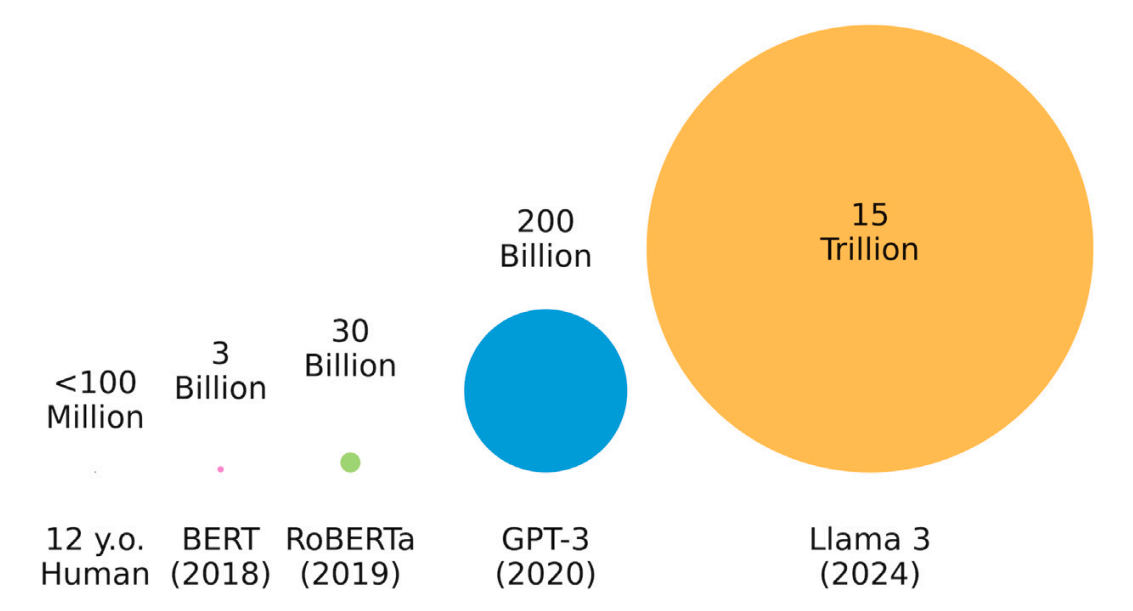
\includegraphics[width=0.99\linewidth]{12Background/scales.png}
    \caption{Mainstream language models are trained on multiple orders of magnitude more word tokens than the amount available to a typical child. \emph{Reproduced from \citet{wilcox2025} under CC BY 4.0.}}
    \label{fig:12-scales}
\end{figure}

\paragraph{Linguistic research.} For decades, language models have been used to study human language learning and processing. For example, \citet{hale-2001-probabilistic} introduced surprisal theory, establishing a groundbreaking connection between the negative log-probability of a word (according to a language model) and real-time human language processing. This finding has been demonstrated repeatedly in ever-more sophisticated language models architectures, correlating surprisal with reading times, eye movements and brain activations \citep[e.g.][]{levy2008expectation, futrell2019neural, futrell2020lossy, schrimpf2021neural}. Early demonstrations that connectionist models can learn grammatical patterns from data alone \citep[e.g.,][]{elman-1990-finding, macdonald1994lexical} revived foundational questions about the \emph{learnability} of natural language \citep{gold1967language}. The increasing capabilities of language models and their success on downstream tasks has motivated research into the internal representations of LMs and assess their ability to learn human-level grammatical generalisations \citep{hewitt-manning-2019-structural, hu-etal-2020-systematic, manning-2020-emergent}.

% maybe fit in a citation for futrell2019neural and dupoux-2018-cognitive

However, there are issues with using LLMs for testing probabilistic theories of language processing. Considering surprisal theory, \citet{wilcox2020predictive} found that language models with a better ability to predict upcoming words are also better predictors of human language processing. However, \citet{shain2024large, oh2024frequency} found that this trend is reversed in LLMs. \citet{wilcox2025} argue that ``bigger is not always better''; LLMs are now such good predictors of language that they no longer provide human-like probability distributions that can be used to further psycholinguistic theories. This is also the case for using LLMs as cognitive models of human language learning. Researchers that advocate for the use of language models as cognitive models highlight the importance of human-like pre-training \citep{linzen-2020-accelerate, baroni-2022-proper,warstadt-2022-artificial,wilcox2025} with a particular focus on the \emph{scale} of data used to train these models. This is illustrated in \cref{fig:12-scales}, which shows that \llama-3 is exposed to hundreds of thousands of times more words than the what humans experiences by the onset of adolescence --- estimated to be 100 million words for children growing up in the United States \citep{gilkerson2017mapping}. Besides scale, there are also concerns that the domain of pre-training data is not developmentally plausible \citep{huebner-etal-2021-babyberta, warstadt2023findings} and that using input representations that do not resemble the sensory signals perceived by humans during language learning confound possible insights gained from using language models as cognitive models \citet{dupoux-2018-cognitive}. 

Motivated by these concerns, the BabyLM challenge was developed to encourage pre-training research with developmentally-plausible corpora \citep{warstadt2023findings}. Participants are challenged to train small LMs on a corpus of 100 million words, using audio transcripts and child-directed domains as source data. However, the challenge uses textual data, and the vast majority of participating systems use subword-based representations. There are similar communities that focus more on the plausibility of the input representation, such as the Zero Resource Speech Challenge, which promotes developing unsupervised methods that learn language directly from audio \citep{dunbar_self-supervised_2022}. This work is discussed further in \writemore.

\paragraph{} The three factors discussed above have contributed to the recent shift toward training smaller language models in domain-specific and developmentally-plausible settings. Yet,within this work, comparatively little attention has been paid to the input representations used by these models. The computational and architectural pressures that originally motivated the adoption of subword units have become so dominant that most research now focuses on the choice of subword model itself (as discussed in \cref{sec:12-subword}), rather than exploring alternative forms of representation.

The BabyLM challenge exemplifies how entrenched subword-based input representations have become. Although concerns about developmental plausibility might naturally encourage the use of auditory or visual representations --- such as the phoneme-based inputs used in early cognitive models (see \cref{sec:12-phonemic}) --- the subword-based representation is the default. The organisers acknowledge that this is a limitation of the framework \citep{wilcox2025}, pointing to both the lack of suitable alternative data and an aim to attract broader participation as reasons for this choice. Indeed, the challenge is motivated not only by the goal of advancing cognitive and psycholinguistic modelling, but also by more practical objectives such as democratising pre-training research and accelerating architectural innovation --- goals for which text-based subword representations are well suited. Nonetheless, developmentally-plausible pre-training remains a promising framework for exploring phoneme-based input representations, as discussed further in \cref{sec:12-plausiblepretraining}.

\section{Subword-based input representation}\label{sec:12-subword}

Modern large language models (LLMs) that operate on textual input rely on subword-based input representations, which offer a balance between generalisability and computational efficiency. In the standard framework, the conversion from raw text to model-ready input is handled by a component known as a \defn{tokeniser}, as implemented in libraries such as \texttt{HuggingFace Tokenizers}.\footnote{\href{https://huggingface.co/docs/tokenizers/index}{huggingface.co/docs/tokenizers/}} A typical tokenisation pipeline comprises several sequential stages:

\begin{itemize}
\item \textbf{Pre-processing:} operations such as lowercasing, accent removal, Unicode normalisation, or character-to-byte conversion
\item \textbf{Pre-tokenisation:} splitting the input into word-like units, often using whitespace and punctuation
\item \textbf{Subword model:} segmenting word-like units into subword tokens using models such as BPE, WordPiece, or Unigram
\item \textbf{Vocabulary mapping:} converting subword tokens into integer IDs for input to the model
\item \textbf{Post-processing:} adding special tokens required by the model (e.g., \texttt{<BOS>}, \texttt{<EOS>}, or segment markers)
\end{itemize}

This pipeline broadly mirrors the classical NLP approach to text processing, although some terminology has shifted: what was once referred to simply as “tokenisation” in traditional NLP is now more precisely termed pre-tokenisation. However, due to the centrality of subword segmentation in modern architectures and minimal pre-processing practices, the terms “tokenisation” and “tokeniser” have become overloaded. In their narrow sense, they refer specifically to the operations of the subword tokenisation model. In their broader sense, they encompass the entire pipeline from raw text to token IDs.

In this thesis, the terms “subword tokenisation” and “subword tokeniser” will be used to refer to the narrow sense, while “tokenisation” and “tokeniser” will be used in the broader sense unless otherwise specified.

% Packaging up these pre-processing steps into a single tokenizer provides convenience, but this has had consequences. In classical NLP, it was an important step to carefully considering the data cleaning operations. For example, removing punctuation... \writemore. The scaling ability of modern LMs has largely shifted the focus to language model architectures and machine learning algorithms, with many models using default tokenisers from Huggingface without considering the impact. This is particularly the case for studies using smaller LMs to study language or acquisition (see \cref{sec:12-babylm}) where subwords in particular may not be an appropriate base unit, nor the orthographic domain if simulating spoken speech. In these cases the default representation is no longer as crucial for performance, yet the convenience of the existing frameworks facilitates its use. 

% The design and availability of this tokenization pipeline has largely been driven by the sheer scaling capabilities of LM architectures, the largest of which are called ``large'' language models (LLMs). Now, the vast majority of language models are distributed on platforms such as Huggingface with an associated tokenizers that consistently process orthographic text, pre-tokenize the text to preserve word boundaries, and return tokens representing subwords.

\subsection{Subword tokenisation methods}

Formally, subword tokenisers can be defined as a tuple $\tokeniser \defeq (\vocab, \detok, \tok)$. The first item in the tuple is the \defn{vocabulary} $\vocab$: a finite set of subwords, each defined as a concatenation $\subword \defeq \ch_i \circ \cdots \circ \ch_j$ of symbols $\ch$ from an alphabet $\alphabet$. The alphabet can be defined as the unique characters appearing in the pre-tokens --- this can be all unique characters appearing in the data (e.g. letters, punctuation and whitespace) or the set of all bytes, if using character-to-byte conversion. Without loss of generalisation, the alphabet is assumed to be bytes.

The remaining components are two functions that map between byte sequences and subword sequences: the \defn{detokenisation function} $\detok\colon \vocab^* \to \alphabet^*$ reconstructs a byte sequence from subwords, by concatenating subwords; the \defn{tokenisation function} $\tok\colon \alphabet^* \to \vocab^*$ performs the reverse mapping and must be injective, satisfying $\chvec = \detok(\tok(\chvec))$.

A common class of subword tokenisers are \defn{bottom-up tokenisers}. These tokenisers choose their vocabulary sequentially, starting from an initial set of symbols (e.g., bytes) and iteratively merging pairs of symbols until a pre-specified vocabulary size is achieved. For example, BPE \citep{gage1994new, sennrich-etal-2016-neural} and WordPiece \citep{schuster-nakajima-2012-voice} are two popular instances of this class.

Training a tokeniser amounts to selecting the tokens to add to the vocabulary by optimising an \defn{objective function} $\obfn$. Selecting tokens is hard, NP-hard: even for simple objectives like compression, selecting the sequence of merges that maximises $\obfn$ globally is NP-complete \citep{kozma-etal-2024-theoretical, whittington2024tokenisation}. Thus, bottom-up tokenisers are typically trained by greedily optimising $\phi$ in a sequential fashion.

Formally, given an initial $\alphabet$ and a corpus $\dataset$, a bottom-up tokenisers learns a sequence of merges $\mergevec$ by greedily optimising an objective function $\obfn$. Common objective functions used by current LMs are the BPE or WordPiece objectives:
\begin{align}
    \bpeob(\merge, \dataset_k) &\defeq 
    \countfn(\lefttoken \righttoken, \dataset_k) \label{eq:bpe_obj} \\
     \wpob(\merge, \dataset_k) &\defeq 
    \frac{
    \countfn(\lefttoken \righttoken, \dataset_k)}{\countfn(\lefttoken, \dataset_k)\,\countfn(\righttoken, \dataset_k)} \label{eq:wp_obj}
\end{align}
where $\countfn(\subword, \dataset)$ denotes the number of occurrences of token $\subword$ in dataset $\dataset$ and the merge $m$ produces a new token from the tokens $\lefttoken$ and $\righttoken$. At each iteration, BPE (\cref{eq:bpe_obj}) selects the most frequent merge pair, while WordPiece (\cref{eq:wp_obj}) selects the merge pair with the largest pointwise mutual information in the dataset.

\begin{figure}[t]
    \centering
    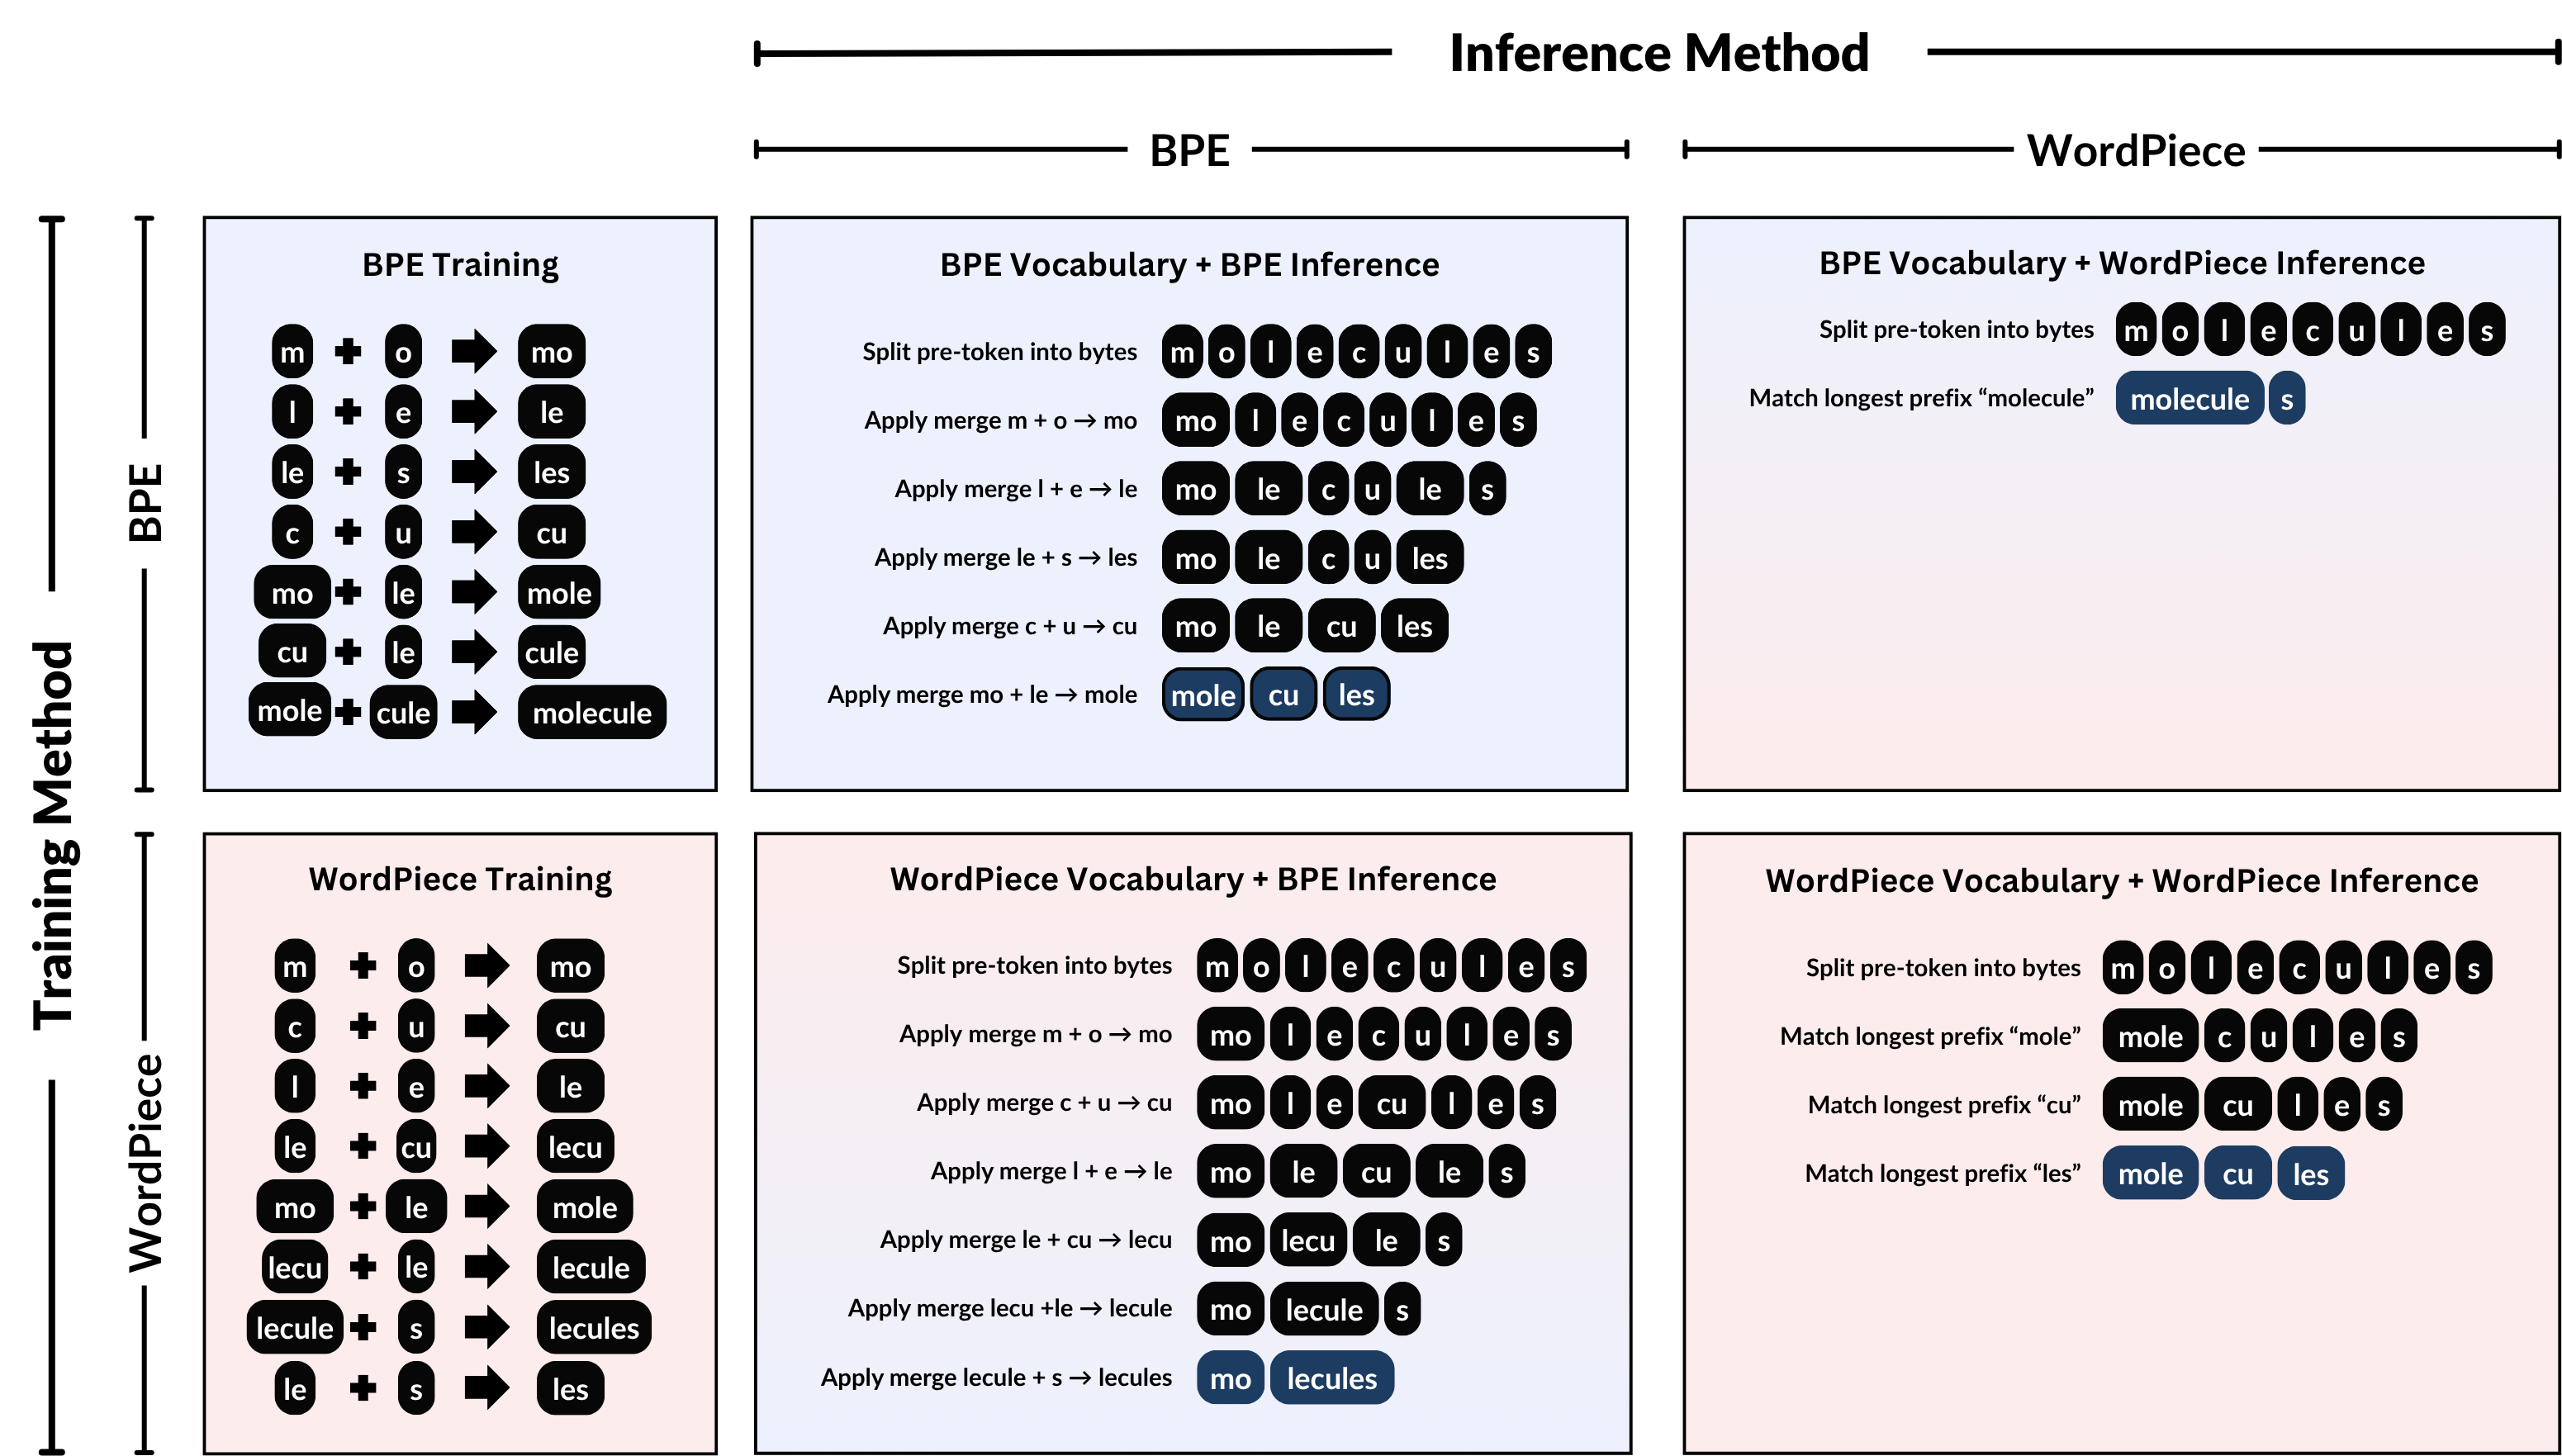
\includegraphics[width=0.99\linewidth]{12Background/tokenisers.png}
    \caption{Comparison of BPE and WordPiece training and inference procedures on the word \ex{molecule}. Merge operations are illustrative and not derived from real training data.}
    \label{fig:12-tokenisers}
\end{figure}

For a given vocabulary, BPE and WordPiece apply distinct tokenisation functions $\tok$ to segment pre-tokens into subword tokens. BPE operates via iterative merging: it begins by splitting pre-tokens into bytes, then greedily applies the merges learned during training. WordPiece uses a longest-prefix matching strategy: for a given pre-token, it recursively identifies and segments off the longest prefix found the vocabulary, repeating this process until the entire pre-token is segmented.

Tokenizer function strategies are also known as \defn{inference methods}. The training and inference methods for BPE and WordPiece are illustrated in \cref{fig:12-tokenisers}. Like their training procedures, both inference methods are greedy and do not necessarily yield the most compressive segmentation for a given vocabulary. For instance, both tokenisers segment \ex{molecules} into three tokens --- ${\ex{mole},\ex{cu},\ex{les}}$ --- even though more compressive segmentations are possible with the respective vocabulary. Because training and inference methods are independent, one can pair the inference method of one subword model with the training method of another, as explored by \citet{uzan-etal-2024-greed}. In \cref{fig:12-tokenisers}, these cross-model pairings yield more efficient two-token segmentations (although note that this is a constructed example for illustrative purposes). 

\Zeb{Maybe talk about SentencePiece as skipping pre-tokenisation}

While BPE and WordPiece are widely used and representative examples of subword tokenisation, many alternative methods have been proposed. A comprehensive review of these approaches lies beyond the scope of this thesis; for a broader survey of subword tokenisation techniques in NLP, see \citet{mielke2021between}.

\subsection{Limitations of subword-based representations}

Several studies exploring limitations of subword-based tokenisers. Evaluating tokenisers is difficult 

\paragraph{Pre-tokenisation.} Splitting words into pre-tokens may not only involve arbitrary decisions about the notion of a ``word'', but also reduce the possible efficiency. SentencePiece \citep{kudo-richardson-2018-sentencepiece}.

\paragraph{Cognitive modelling.} \citep{beinborn-pinter-2023-analyzing}, limiting their value for psycholinguistic research \citep{giulianelli-etal-2024-proper} less effective than character-based tokens for learning word structure \citep{bunzeck2025subwordmodelsstruggleword}. \citet{fan-sun-2023-constructivist} argue for the necessity of a constructivist approach to tokenization, training an LSTM model on gold labelled data to tokenise text into morphemes, claiming that this enables the training of computational models that more closely align with language comprehension and acquisition.

\paragraph{Morphological alignment.} \citet{bauwens-delobelle-2024-bpe} note that BPE can often concatenate partial morphemes, preventing the formation of morphemes and introduce BPE-knockout, a method that removes problematic subwords, which improves morphological alignment. Similarly, \citet{asgari2025morphbpe} also propose a morphology-aware extension of BPE that maintains compression while providing better morphological alignment across several languages. Similarly \citet{kildeberg2025sm} for Dutch, \citet{nzeyimana-niyongabo-rubungo-2022-kinyabert} for Kinyarwanda, \citet{erkaya2022comprehensive} for Turkish, \citet{pan2020morphological} Turkish and Uyghur

\paragraph{Multilingual modelling.} \citep{limisiewicz-etal-2024-myte} as morphological tokeniser. Nevertheless, the over-segmentation problem still
exists even at the byte level, as byte sequences for
single characters are overly long for many nonLatin script languages

\paragraph{Intermediate merges.} 


\paragraph{Evaluation.} Evaluating subword tokenisers is difficult since comparing a suite of tokenisers would require pre-training language models from scratch using each, and the scaling laws mean that downstream effects may only not be apparent unless large models are used \citep{wei2022emergent}. Typically, studies address this by trying to find \emph{intrinsic} properties (e.g. properties that can be computed without a language model) that correlate with \emph{extrinsic} behaviour (performance of language models), allowing later studies to use these metrics as a proxy. 

However, despite the number of criticisms and intrinsic properties discovered, it remains unclear what properties are desirable in a tokeniser. Compression certainly helps make language modelling efficient, but morphological alignment or cognitive alignment might be preferable when using the language model for cognitive modelling or linguistic research.
In general, just as the ``one size fits all'' paradigm for LLMs is not appropriate for all domains (as discussed in \cref{sec:12-domainspecific}), there is unlikely to be a subword tokeniser suitable for all purposes, and subwords themselves may not be the appropriate representation for certain domains. Instead, these limitations should encourage researchers to consider the input representation more carefully depending on the task and domain being modelled.

\subsection{Alternative input representations}

\Zeb{Briefly survey speech models, pixel tokenisation etc. but probably don't go into too much detail.  Maybe patches work goes here as well.}

\paragraph{Patching.} The quadratic cost of self-attention and the high per-position cost of large feed-forward networks have limited the ability of LLMs to model very long sequences. To address this, \citet{yu2023megabyte} introduce the concept of \defn{patching}. In this framework, byte embeddings are concatenated to form patches—units that roughly correspond to subword token, which are then processed by a global transformer. The resulting patch representations are decoded by a local transformer, which can even model raw audio. \citet{pagnoni2024byte} extend this idea to latent patches: instead of using fixed-length windows, the model segments variable-length patches in a latent space, with boundaries determined by the next-byte entropy estimated by a byte-level model. Overall, patching aims to improve the computational efficiency of language models beyond what subword tokenisation alone can achieve \citep{shao2025beyond}.

\paragraph{Character and byte-level.}
Despite the higher computational costs associated with character-level tokenisation, it has been actively explored as an alternative to subword units, motivated in part by the desire to build models that are more robust to noise and better capture morphological variation \citep{gupta2019character}. \citet{al-rfou_character-level_2019} show that sufficiently deep transformers can match the performance of subword- or word-level models, suggesting that the transformer architecture is largely agnostic to input granularity. \citet{libovicky-fraser-2020-towards} further demonstrate that this depth can be reduced by fine-tuning subword-level models.
This line of work also includes byte-level models, such as ByT5 \citep{xue-2022-byt5}, which operate directly on raw bytes—a natural choice when following the "principle of modelling the smallest meaningful units in the data" \citep{graves2013generating}. Character- and byte-level approaches are often described as \emph{token-free} \citep{clark-2022-canine, xue-2022-byt5}, although \citet{mielke2021between} argue that this label is misleading: these models still rely on a fixed, predefined tokenisation scheme—one that simply aligns with how data is conventionally stored on disk.

\Zeb{Perhaps the next few (previously input representation comparisons) could be moved to modelling chapter as related work.}

To the best of our knowledge, a full systematic comparison of the three input transformations has not yet been conducted.  \citet{hahn-baroni-2019-tabula} investigated the effect of removing word boundaries and using a word-level or character-level tokenization, evaluating on several psycholinguistic benchmarks. However, they only used graphemic text from Wikipedia and did not ablate the two transformations, only comparing a word-level model (with word boundaries) to a character-level model (without word boundaries). \citet{nguyen-2022-word-boundaries} extend this work, comparing character-level graphemic input (with and without word boundaries) to character-level phonemic input (with and without word boundaries) by training on the Librispeech corpus \citep{panayotov2015librispeech}. They also compare larger units of tokenization (BPE and word-level) for both graphemic and phonemic text, but only with word boundaries included, missing out on several key combinations. 

In our work, we provide a complete comparison of these three input representation transformations by considering all combinations, leading to new input representations that have not been studied before (such as subword tokenization trained without word boundaries). We also use a larger model than previous work, a 12-layer transformer rather than a 3-layer LSTM.

%Another simple heuristic for processing text to be more speech-like is to remove word boundaries. At the simplest level of approximation, some past efforts have studied the effects of removing word boundaries from language models \citep{hahn-baroni-2019-tabula, nguyen-2022-word-boundaries}, finding that LSTM-based models see a marked decrease in performance on several psycholingustic benchmarks. 

% However, these architectures were developed for downstream tasks and not for linguistic theories \citep{baroni-2022-proper}. Before using such models, we must establish the extent to which using standard orthographic text gives language models an advantage over input representations that more closely mimic human speech. 

%However, underlying these approaches is a concern that language models trained under common paradigms may not be scientifically sound for providing insights into human language acquisition. This is because the development of language models is driven by downstream performance on popular tasks rather than being grounded in linguistic theories \citep{baroni-2022-proper}. The recent explosion in the size of language models has further complicated comparisons between human and neural network language acquisition. \citet{warstadt-2022-artificial} argue that to draw valid conclusions about human language acquisition from neural networks, the trained models should not possess any advantages over humans. Similarly, \citet{dupoux-2018-cognitive} proposes that machine learning models should use raw sensory signals perceived by humans (e.g., sound waves) as inputs to remove confounding variables that make interpreting their behaviour as models of language acquisition challenging. Similarly to how the BabyLM challenge reduces the training set to a reasonable size, the Zero Resource Speech Challenge involves developing unsupervised methods that learn language directly from audio \citep{dunbar_self-supervised_2022}. We discuss this paradigm further in \cref{sec:14-audiomodels}.

\subsection{Character-based Language Models}

The use of characters as the input representation, rather than words or subwords, has been extensively explored. Character-level language models offer a simplified input stream compared to the standard approach of training on learned susword tokens. Many studies have developed specialised architectures to train language models on characters \citep{jozefowicz2016exploringlimitslanguagemodeling, kim2016character, ma-etal-2020-charbert, al-rfou_character-level_2019} while other approaches seek to establish `token-free' training regimes to eliminate the need for subwords entirely \citep{clark-etal-2022-canine, xue-2022-byt5}.

Another alternative input representation is to split words into morphemes, which provide theoretical benefits over subwords and have their own analytical and practical benefits particularly for morphologically rich languages \citep{ustun-etal-2018-characters, nzeyimana-niyongabo-rubungo-2022-kinyabert, fan-sun-2023-constructivist}. Mapping orthographic text to morphemes continues to be a challenging task, requiring dedicated systems trained on labeled corpora \citep{batsuren-etal-2022-sigmorphon} and we do not consider morphemes in this work.

% \Zeb{Give background on what LMs use by default. Define as subwords + orthographic + pre-tokenization.}

% \Zeb{Define tokenizers more formally and discuss BPE and WordPiece etc and pointing to some surveys about these methods. Greed is all you need method.}

% \Zeb{Plausibility of subwords, issues in certain languages, misalignment etc. Superword paper as an alternative to word boundary-based pretokenization. Morpheme-aligned alternatives that never caught on. Many alternative approaches. Character-level models and byte-level models. Attempts to go `token-free' but byte-level still an arbitrary token choice.}

% \zeb{Change this to be about the tokens rather than the tokenizers}
% \begin{enumerate}
%     \item process written (orthographic) text,
%     \item pre-tokenize the text to preserve word boundaries, and
%     \item split pre-tokenized into tokens that represent subwords.
% \end{enumerate}

% The combination of these three features will henceforth define the \textbf{default input representation}. Now, the vast majority of language models are distributed with an associated tokenizer. The tokenizer converts noisy text to unique token IDs, which are fed through the model, which produces contextual embeddings. Auto-regressive LMs are trained with a next-token prediction objective, allowing them to generate text one token at a time, which the tokenizer can convert back into readable text. Alternatively, the contextual representations are directly used, or the model is fine-tuned on a downstream task involving labelled data. There are countless variations to this setup in modern NLP but the vast majority use tokenisers...

% In recent years, tokenization has become an increasingly popular topic, with the default configurations of popular tokenizers often critiqued and analysed, and many studies proposing improvements and alternatives to existing tokenizers. An overview of this work is provided in \cref{sec:12-default}. Despite this scrutiny, the focus is still on tokenizers that produce the default input representation. 

\section{Phoneme-based input representation}\label{sec:12-phonemic}

Several language models have been trained with phonemic input \citep{sundararaman-2021-phonemebert, gale-etal-2023-bort} but it remains a challenge to do so due to the lack of large phonemic corpora. While a number of well-known speech-based datasets include phonemic transcriptions, such as Switchboard \citep{godfrey1992switchboard} and TIMIT \citep{garofolo1993darpa}, these datasets are small compared to the trillions of tokens contained in standard language model pre-training corpora \citep{elazar-2024-redpajama}. The majority of works that use phonemic representations typically rely on grapheme to phoneme conversion tools \citep{bisani-2008-g2p, hasegawa-2020-g2pmultilingual} to generate coarse phonemic transliterations of text data.

It is also a challenge to evaluate the broad capabilities of language models trained with phonemes, as most benchmarks assume a graphemic representation, even some that assess phonological knowledge \citep{suvarna-etal-2024-phonologybench}. One benchmark that assesses both the syntactic and phonological capabilities of language models is BabySLM \citep{lavechin}. %One distinguishing advantage of this benchmark is that it can be applied to models trained on either graphemes or phonemes.
We discuss this benchmark further in \cref{sec:14-effect}.

\citep{nguyen-2022-word-boundaries,bunzeck2024graphemes}

\subsection{Motivation and linguistic rationale}

Cross-linguality, alignment with speech, abstraction

Why model phonology with language models?

Why phonemes rather than orthographic input?

Phoneme representations as more universal, cognitively plausible, and appropriate for speech-based modelling

Introduce the tension: LMs are often tested on phonological knowledge despite being trained on orthographic input.

\subsection{Implementation of phoneme-based input}

%The construction of phoneme-based input typically involves a grapheme-to-phoneme (G2P) conversion step, followed by tokenisation over the resulting phoneme sequence. In this work, G2P conversion and dataset construction are handled by a new tool and dataset, introduced and described in detail in Chapter [X]. Here, we provide only a high-level overview to situate the phoneme-based input representation within existing practices.

%Large language models are typically trained on written text using tokenizers that split the text into subword units. By contrast, studies that train models using a phoneme-based input representation tend to use tokenizers that produce a token for each individual phoneme, akin to character-based language models. Often, phonemes are fed to a model in a sequence that does not contain word boundaries, as utterances tend to be produced continuously, with no pauses between individual words. 
% The standard input representation for training large language models consists of written text split into subword units. By contrast, studies that train models using a phonemic input representation tend to split words into individual phonemes, without word boundaries (as spoken utterances are produced continuously, without clear pauses between words).



Very brief summary of how phoneme inputs are constructed

High-level G2P overview, mention of boundary decisions, tokenisation granularity

Forward-reference your tool and dataset in the next chapter

Possibly add a short note on typical phoneme vocab size and training behaviour


Soon after word2vec, \citet{ma2016learning} presented a model that learned phoneme embeddings using the  a word segmentation task

\subsection{Word segmentation}

Phoneme-based models in word segmentation, especially in child-directed speech

Compare to subword segmentation in LLMs

Discuss what phoneme-level segmentation reveals about inductive biases or learning difficulty

Unlike in written text, where lexical units are separated by spaces and punctuation, spoken communication consists of continuous utterances with no clear demarcation of words (see e.g. \citet{cole1980model}). Somehow, without a lexicon to consult, children are able to segment speech into words and phrasal units by the age of six months \citep{Jusczyk1999infants}. How children learn to segment words and bootstrap their lexicon is known in psycholinguistics as the \emph{word segmentation problem}, and statistical learning experiments have established a wide variety of statistical cues which children may use to segment speech \citep{Cutler1987, gleitman1988learning, Jusczyk1993stress, Saffran1996distributional, Jusczyk1999allophonic, Suomi1997}.


When using a phonemic input representation to model speech, word boundaries are not typically included, as word boundaries are not explicitly marked in the speech stream. The phoneme stream representation (i.e.,\ the combination of all three transformations) is the typical representation for word segmentation studies, where the task is to learn word boundaries without supervision \citep{Brent1999}. A wide variety of statistical, dynamic programming and neural approaches have been applied to the task, with consequences for acquisition research and low-resource language modeling \citep{Blanchard2010, Coltekin2017, algayres_dp-parse_2022, goriely2023word}.


\citet{christiansen1998learning} later used an SRN to segment speech by using the probability of an \emph{utterance} boundary, rather than prediction-error, to place word boundaries. This followed previous work suggesting that children could use utterance boundaries to bootstrap their lexicon \citep{aslin1996models} and is a cue used in the models of \citet{ccoltekin2014explicit, goriely2023word}.


Particularly influential were the experiments of \citet{Saffran1996learning}, who established that 8-month-old children use distributional information to segment speech, specifically noting that low conditional probability %\footnote{In their study, the calculation is called ``transitional probability''.}
between two adjacent syllables often indicated a word boundary. These experiments inspired the development of computational models proposing cognitively plausible learning mechanisms for word segmentation, most of which are based on the principle that units within words are far more predictable than units across word boundaries \citep{harris1955}. Many models draw on \citet{Brent1999}, who used unigram statistics to segment speech, with later models using higher-order n-grams \citep{Venkataraman2001}, incorporating phonological constraints \citep{Blanchard2010} or leveraging prior distributions over word frequencies and phonological shapes \citep{Goldwater2009}. Other models explicitly calculate several statistical cues at each potential word boundary and combine cues using a majority voting framework \citep{ccoltekin2014explicit, Coltekin2017, goriely2023word}. Each cue provides a signal over the utterance (as illustrated in \cref{fig:15-example}) with peaks in each cue indicating a potential boundary. 

% Some models leverage n-gram statistics \citep{Brent1999, Venkataraman2001}, some  Blanchard2010, Elsner2017, Coltekin2017}. Many of these models were evaluated on 10,000 utterances from the Bernstein-Ratner \citeyear{bernstein1987phonology} corpus in CHILDES, transcribed phonemically by \citet{Brent1999}, who also established the evaluation metrics for word segmentation performance (see \cref{sec:15-evaluation}).
%Brent also established the typical metrics used to evaluate word segmentation performance (see \cref{sec:15-evaluation}) and phonemically transcribed 10,000 utterances from the Bernstein-Ratner \citeyear{bernstein1987phonology} corpus in CHILDES which continues to be used to evaluate segmentation models. 

\subsection{Phonological experimentation}


\Zeb{More recent studies that use LMs to study phonology by using tiny LMs that train just over word types rather than tokens in context. Conclude that there have been few attempts at training cross-lingual LMs on naturalistic running text to get a model of phonology for each language.}

Since their inception, language models have been used to study the structures of language and explore mechanisms that humans may use to learn them. 

Early ``connectionist'' language models were trained on sequences of letters or phonemes, often using developmentally plausible data in order to explore theories of word learning and phonology \citep{seidenberg1989distributed, norris1994shortlist, coltheart2001drc}. 


Connectionist/early models of phonotactics and processing

LSTM/phoneme-level language models (e.g., phonotactic generalisation, nonce-word acceptability)

Tie back to phoneme input’s usefulness for probing phonological knowledge


Here, we are interested in evaluating models that train directly on individual phonemes, without word boundaries. When trained on individual words, phoneme LMs have been used to study the acquisition of morphological rules \citep{kirov-2018-recurrent} and compare phonotactic complexity across languages \citep{pimentel2020phonotactic}. When trained on running text, phoneme LMs have been used for text-to-speech \citep{li-2023-phoneme-level-bert} and lyric generation \citep{ding-2024-songcomposer}. When compared to grapheme-based models on standard linguistic benchmarks, phoneme models slightly under-perform \citep{nguyen-2022-word-boundaries, bunzeck2024graphemes} but this could be attributed to pre-processing, punctuation and the fact that LLM architectures and evaluation sets have been optimised for written text \citep{goriely2024babble}. Despite the benefits of phoneme-based training, phonological evaluation is limited, and few phoneme LMs exist beyond English. \citet{goriely2025} trained phoneme LMs on child-directed speech across 11 languages, but were only able to use an English benchmark for studying how phonological and syntactic knowledge scales in phoneme LMs. 


\subsection{Phonological evaluation of transformer language models}

Overview of studies evaluating phonological knowledge in LLMs

Key point: many of these models are trained on orthographic input, yet tested on phonological tasks (e.g., stress assignment, phonotactic acceptability)

Argue that this introduces a representational mismatch

Suggest that phoneme-based LMs offer a more principled alternative for such evaluations, but note that work in this area remains limited due to lack of G2P tools and phonemically annotated corpora.


\Zeb{Discuss prior evaluation used to evaluate language models for phonological knowledge. Possibly start with wider background looking at how people evaluate LMs for knowledge of linguistic structure. Discuss phonologybench as the opposite of what we're looking for. BabySLM is more relevant, discussed in the next section.}

While many studies have explored the representations learned by phoneme LMs trained on individual words, there are very few benchmarks for phoneme LMs trained on running text.

One method for testing phonology is to use minimal pairs of words and pseudowords as a lexical decision task. One benchmark that uses this approach is BabySLM \citep{lavechin}, which provides a lexical decision metric for phoneme LMs or speech LMs (which learn directly from audio) using a vocabulary based on child-directed speech. \citet{bunzeck-etal-2025-small} use a similar approach in order to compare grapheme LMs to phoneme LMs. They also use two probing tasks to examine the representations of sentences; age prediction and rhyme prediction. %These studies only test English models, in part due to the lack of phoneme LMs in other languages, but also due to a lack of resources for constructing phonological tasks. For example, they both use \texttt{wuggy} \citep{keuleers2010wuggy} to generate pseudowords, which only supports three languages for phonetic pseudoword generation.


%Very few methods for measuring phonological evaluation of LLMs. PhonologyBench is one example but is based on prompting for very large language models trained on orthographic text, limiting analysis of representations learned for individual phonemes. BabySLM provides a lexical decision task, more closely relating language models to psycholingustic studies of human preference. \citet{bunzeck-etal-2025-small} use a similar test, also exploring rhyme prediction and age prediction as phonological tasks. These studies all only explore English phonology due in part to the lack of phonemic data in other language \citep{goriely2023word} as well as a lack of resources for constructing phonological tasks. For example, BabySLM uses Wuggy to generate pseudowords but Wuggy only supports three languages for phonetic pseudoword generation.

PhonologyBench \citep{suvarna-etal-2024-phonologybench} is a benchmark that uses prompts to test chat-based English LLMs. However, by using prompts, they treat phonology as an emergent ability tested through metalinguistic judgment, an evaluation strategy which \citet{hu2023prompting} argues is inferior to using quantities directly derived from a model's representations.  

These benchmarks also only test English models, in part due to the lack of phoneme LMs in other languages, but also due to a lack of resources for constructing phonological tasks. For example, pseudowords are typically generated using \texttt{wuggy} \citep{keuleers2010wuggy}, which only supports three languages for phonetic pseudoword generation. An example of language-independent evaluation of phoneme LMs is the phonetic feature probe used in \citet{goriely2025}, which only requires feature vectors for each IPA symbol. The word segmentation task requires no language-specific data, only utterances labeled with word boundaries. 

% Compared to models trained on orthographic text or raw audio, few studies training with phonemes. Models based on BERT have shown that training with phonemes can be useful for downstream tasks. In comparison studies, grapheme models slightly outperform phoneme models \citep{nguyen-2022-word-boundaries, bunzeck2024graphemes} but this could be attributed to preprocessing differences, punctuation and the fact that typical LLM architectures have been optimized for written text \citep{goriely2024babble}. As with phonological benchmarks, few phoneme LMs exist for languages other than English. Here, we release phoneme LMs trained on the 31 languages in \ipachildes...


\subsection{Why not use audio-based representations?}\label{sec:12-whynot}

%CHAT: In addition to orthographic and phoneme-based inputs, recent advances have produced language models operating directly on audio signals. Models such as wav2vec 2.0 and HuBERT learn speech representations end-to-end from raw waveforms, capturing acoustic and phonetic features implicitly. While these models excel in speech recognition and generation tasks, they require vast speech corpora and computational resources. Phoneme-based input representations offer a complementary approach, providing a linguistically interpretable symbolic abstraction that facilitates detailed phonological analysis and modeling with relatively modest data and compute. This thesis focuses on phoneme-level representations to leverage these advantages, while acknowledging the ongoing importance of audio-based models.
%This is revisited in discussion....

% CHAT: While some studies evaluate the phonological competence of large language models, these models are typically trained on orthographic input, creating a potential mismatch between the representational format and the linguistic phenomena being tested. Phoneme-based input representations offer a more direct mapping to the phonological domain and may yield models whose inductive biases better align with phonological generalisation. However, the use of such representations remains relatively rare, in part due to resource limitations — an issue addressed in Chapter [X].

% \Zeb{Combine cross-linguistic work here with phonological evaluation?}

% \Zeb{Some statement here about potential of phoneme tokenisation and the fact that alternative input representations are largely under-studied in NLP, due to the convenience of the default one. Maybe here go into the historical use of the input representation and that it has been vastly understudied. }

% \Zeb{Formal definition of what I mean by the phonemic input representation. This is where the three transformations are described. Similar to character-level. Maybe here worth going more into detail with character-level models and tabula rasa model.}

% %\subsubsection{Practical uses of the phonemic input representation}

% \Zeb{Survey of methods using phonemes. Briefly discuss how important phonemes were for speech recognition technology but now a lot of that is end-to-end. Discuss more recent uses in LMs. End by stating maybe we're resource limited, as discussed in \cref{chapter:resources}}

% \begin{figure}[t]
%     \centering
%     \includegraphics[width=0.99\linewidth]{example-image-b}
%     \caption{The phrase ``example phrase'' encoded using the default input representation compared to the phonemic input representation.}
%     \label{fig:12-representation}
% \end{figure}

% An alternative to the default input representation, and the topic of this this thesis, is the \textbf{phonemic input representation}. This is defined in contrast to above as:

% \begin{enumerate}
%     \item process phonemic text,
%     \item do not preserve word boundaries, and
%     \item split text into tokens that represent individual phonemes.
% \end{enumerate}

% A major use of the phoneme representation is phonological experimentation. This includes connectionist models of language processing, computational models of word segmentation and word-level phonotactic models, as discussed in \cref{sec:12-phoneval}. A practical use was speech recognition technology. Was important to create phoneme-level models along with language models in a complicated system to do TTS, STT, voice recognition, language recognition, etc. Many resources were built to support this, many phonological datasets. A detailed analysis of existing phonological resources in given in \cref{chapter:resources}.

% Despite this history, less work exploring phoneme representation in modern NLP landscape. One reason could be that the scaling abilities of LLMs have favoured text, which is more readily online and regularly scraped. Speech technology has also largely moved to end-to-end directly from/to audio, without needing discrete phoneme models.

% Yet, phoneme LMs do offer some practical benefits which have been explored, \writemore. There are also analytical benefits, as discussed in \cref{sec:12-phoneval}.

% % One reason could be a lack of resources, which is the topic of \cref{chapter:resources}. A benefit of exploring alternative input representations is to ablate the effect of each of the features of the default representation, as explored in \cref{chapter:modelling}. The cognitive aspect... \cref{chapter:phonology}... and could improve tokenisation methods... \cref{chapter:infotokenization}.

% Phoneme language models. Many word-level models to study phonology. Very few examples of running text. Some examples of working with audio directly, as discussed in the next section.

% Phoneme representation could be compared against default representation along three axes. There is some work comparing these effects. Several studies have challenged (3) by demonstrating that character-based or byte-based models can still be effectively utilised in language models \addcites. These argue to be "token free" but according to \addcites is still an arbitrary subword representation. A few studies have challenged (2) by relaxing the word-boundary pre-tokenization constraint to produce `superword' tokens \addcites or explore the effect of removing whitespace altogether to achieve a `tabula rasa' input representation \addcites but still orthographic text. Finally, Bunzeck paper. \cref{chapter:modelling} properly compares these to establish the effect of the phoneme representation in modern language models.

\section{Developmentally-plausible pre-training}\label{sec:12-plausiblepretraining}

\citet{salhancopil2025} for a discussion on how BabyLMs can be used for investigating linguistic theories. 

\Zeb{Three aspects: small language models good for low-resource or domain-specific work (languages), researching human language learning, and architecture research within academic budgets. }

- 1. LLMs are not actually appropriate for certain domains. In some cases, pre-training is more effective and cheaper than fine-tuning. E.g. humanities

- 2. This is especially the case in multilingual modelling... where small language models...

- 3. LLMs also not appropriate for work using LMs to study human language acquisition or processing. Using NNs to study these date back to ..., where phoneme models were used, as discussed in \cref{sec:12-phonemic}. Later work has drawn comparisons between LM pre-training and human processing and learning, but use unrealistic data in terms of scale and size. This has inspired training small models on developmentally-plausible corpora, so-called `BabyLMs' as popularised by the BabyLM challenge \addcites. However, they do not address the other developmental concern, that the subword-based representation may not be appropriate for this line of research --- in part, this is because these representations have become so standardised that they feared losing participants by exploring more plausible domains (see \citet{wilcox2025}). Additionally, the challenge also has wider goals of democratising LM research and exploring data-efficient pre-training methods, which could clash with using a developmentally-plausible input representation.


\Zeb{Idea that ``simulations must closely emulate real-life situations by training on developmentally plausible corpora'' in order to gain insights both about what language models can learn, and improve understanding about how infants learn language. Clearly could be valuable insights for phonology in this area.}

\Zeb{Early example is BabyBERTa paper, who trained on a version of AOCHILDES. Briefly discuss findings and criticisms.}

\Zeb{Later, BabyLM challenge created a framework for training and evaluting such models. Still motivated by developmentally plausible data, but still using default input representation. Findings more about architectures for low-data than specifically for insights into human learning. This framework provides a good way of testing this size model.}

\Zeb{Finally, BabySLM paper, which focused more on speech models. They also trained models on portions of CHILDES, including AOCHILDES, as well as Seedlings, an audio dataset, and compare speech, phonemes and text as input representations.}

\Zeb{Besides BabySLM and Bunzeck papers, very few examples of phoneme-based training on developmentally-plausible data, possible due to resource limitations (see \cref{chapter:resources}). However, these papers provide a useful starting point for establishing whether phoneme-based training is plausible and the datasets and evaluation criteria described below are leveraged in this thesis..}

\Zeb{Should mention \citet{huebner_structured_2018} as an early example of modelling child-directed speech using SRNs, LSTMS and skip-gram.}

\Zeb{Review \citet{wilcox_bigger_2025} and Suchir's paper for wider position pieces on the role of babylm for wider research.}

\Zeb{BabyLM framework is appropriate for two reasons. Firstly, the scale: it's appopriate for academic budgets, phoneme models can be useful for low-resource, and phoneme data is too limited for larger scale models (see next chapter). Secondly, the developmental/analytical angle. These models have been branded as useful for cognitive research due to the developmental plausibility. Phoneme representation so far has mostly been used for analytical purposes, so using develpmentally plausible framework is logical - and using the phoneme representation provide an additional aspect of plausibility beyond written text and exploration is worthwhile.}

Besides low-resource languages, pre-training also more efficient and effective than fine-tuning for domain-specific. For example, humanities language transfre \citep{fittschen2025pretraininglanguagemodelsdiachronic}. Overall, we are seeing a shift away from the LLM framework back towards domain-specific models. But in that time, subword representation is still so entrenched... especially due to tokenisation packages. 


Training models on such little data (here, only 500 thousand words) may be considered atypical in the modern NLP landscape, but questions of developmental plausibility have led to an increased interest in pretraining with limited data. For instance, the BabyLM workshop series challenges participants to train smaller models on data that is limited by both scale, 10--100 million words, and by domain, with the pre-training corpus including data from CHILDES, among other child-centered corpora \citep{warstadt-2023-babylm-findings, hu-etal-2024-findings}. Such limitations have led to the development of new architectures \citep{georges-gabriel-charpentier-samuel-2023-layers, charpentier2024gpt}, motivated cognitively-inspired pre-training strategies \citep{huebner-etal-2021-babyberta, martinez-etal-2023-climb} and allowed for gaining insights into human learning \citep{yedetore-etal-2023-poor}. The majority of this work has centered on English. Exceptions include \citet{capone2024babies, shen2024bambino}, who train Italian monolingual and bilingual models, respectively, \citet{yadavalli2023slabert} who use data from five language in CHILDES to explore second language acquisition theories (but only train an English LM) and \citet{salhan-etal-2024-less}, who use age-ordered data from four languages in CHILDES to explore fine-grained curricula inspired by language acquisition.

\subsection{Datasets}

\subsubsection{The CHILDES database}

\Zeb{Describe CHILDES. Discuss people who have done language modeling with CHILDES (e.g. BabyBERTa).}

The Child Language Data Exchange System (CHILDES) is a repository of child-centred data originally developed with the aim of preserving and standardising data used for child language development research \citep{macwhinney1985child}. The project later grew into TalkBank, which contains over 1.4TB of transcript data and 5TB of associated media data across several ``banks'' \citep{macwhinney_understanding_2019}. Each bank focuses on a different area of human communication, with a general focus on spoken communication, with the CHILDES banks now containing child-caregiver interactions in over 40 different languages thanks to the efforts of hundreds of contributors over the last 40 years. 

CHILDES is an extremely valuable resource for research on child language development and has led to many thousands of published articles since its release. Due to the commitment to open-data sharing, the influence of these resources has also extended to other fields of research. For instance, in a recent assessment on the impact of the TalkBank project, \citet{bernstein_ratner_augmenting_2024} noted that a corpus she had contributed to CHILDES --- originally collected to study the acoustic features of child-directed speech \citep{Ratner_1984} --- was still leading to new insights forty years later:
\zeb{Probaby worth mentioning that this became the BR corpus for word segmenation.}
\begin{quote}
The corpus has been further used to test models of unsupervised induction of grammar in machine language learning \citep{glushchenko_programmatic_2019}, a prospect not remotely envisioned during the original study, when data were collected on reel-to-reel analog tapes, and acoustically analyzed using a dedicated mainframe computer that had to be booted with punched paper tape.
\end{quote}

For researchers seeking developmentally-plausible corpora to use as pre-training data for language models, CHILDES is a natural fit. For instance, BabyBERTa was pre-trained on the AO-CHILDES corpus (Age-Ordered CHILDES, \citep{huebner2021using}). AO-CHILDES contains approximately 5M words from the North American English sections of CHILDES. Specifically, it contains all utterances involving children aged 0 to 6, sorted by child age, with non-adult speech removed (thus simulating the theoretical input received by a child). In their study, \citet{huebner-etal-2021-babyberta} were interested in the outcome of pre-training BabyBERTa on AO-CHILDES compared to Wikipedia (which was considered a more representative dataset for NLP at the time). Using a linguistic benchmark based on BLiMP (see \cref{sec:12-blimp} below), they found that BabyBERTa achieved a higher accuracy when trained on AO-CHILDES, that the choice of corpora had an effect across the pre-training corpus and that ordering multiple corpora by grammatical complexity could `scaffold' learning. These findings validated the importance of using developmentally-plausible corpora for BabyLM research and the scaffolding results were a precursor of many of the curriculum learning approaches taken in the first edition of the BabyLM challenge \addcites.


Maybe cite \citep{padovani2025child} as contradicting huebner in terms of CDL scaffolding generalisability in LMs.

\Zeb{Insert other examples of language modelling with CHILDES}

\Zeb{Insert a few phoneme examples of language modelling with CHILDES, discuss PhonBank}

\subsubsection{The BabyLM dataset}

\Zeb{BabyLM dataset description. Note that they wanted to reach 100M words, which they couldn't just do with CHILDES. Can slightly criticise, not quite developmentally plausible but more so than web-scraped corpora (maybe show figure comparing CHILDES, BabyLM and Pile). Maybe briefly mention other cognitively plausible datasets that have sprung up recently, like German BabyLM, KidLM, storybooks, chat-gpt generated data, future BabyLM multilingual.}

\subsection{Evaluation metrics}

Below are a description of the main benchmarks used in this thesis to evaluate LMs. 

\subsubsection{BLiMP}\label{sec:12-blimp}

\subsubsection{GLUE}

\subsubsection{BabySLM}


\section{Summary}

\Zeb{Go back to research questions. Need to establish whether resources exist. Need to do a thorough comparison of input representations and determine how to do language modeling with phonemes. Need to see what insights can be gained from phonological experimentation with such models. BabyLM framework gives good start to use for this stuff, but still limited ways to evaluate phoneme LMs.}

- 4. BabyLMs provide a very suitable framework for exploring the use of a phonemic input representation. Firstly, scale of data is similar. Past phoneme LMs trained on datasets similar in size to BabyLM and not much data for training LLMs with phonemes. Even finding enough data for LMs is an issue, as thoroughly explored in \cref{chapter:resources}. Thus, using evaluation designed for models at the same scale is ideal for asserting the feasibility of phoneme-based training with LMs, as explored in \cref{chapter:modelling}. Secondly, work using BabyLMs to explore language acquisition have not considered the use of a more developmentally-plausible input representation, and work that does use phonemes for phonological research have not used a developmentally-plausible framework --- thus using a phoneme-based representation within a developmentally plausible framework could enhance both lines of research, both for using LMs for language acquisition research and for improving phonological research with better LMs; experiments conducted in \cref{chapter:phonology}.